\section{Equazione semiclassica di Boltzmann}
Nello studio di una qualsiasi nanostruttura, è necessario mettere a contatto questa struttura con i dispositivi di misura macroscopici. Tipicamente, ciò viene fatto strutturando elettrodi molto più grandi dei sistemi studiati e mettendoli in contatto con questi ultimi. Un tale elettrodo funge da serbatoio ideale (sia termico che di particelle) per gli elettroni. Consideriamo quindi un sistema mesoscopico\mn{Per mesoscopico si intende un sistema di dimensioni intermedie tra quelle microscopiche e quelle macroscopiche. Possiamo quindi dire più semplicemente che tale sistema ha dimensioni piccole.} composto da un conduttore (ad esempio un metallo, un semiconduttore o un isolante topologico) in contatto con due serbatoi $L$ ed $R$, di dimensioni macroscopiche che possono fornire sia cariche (più precisamente elettroni) che energia, come in figura:
\begin{figure}[H]
   \centering
    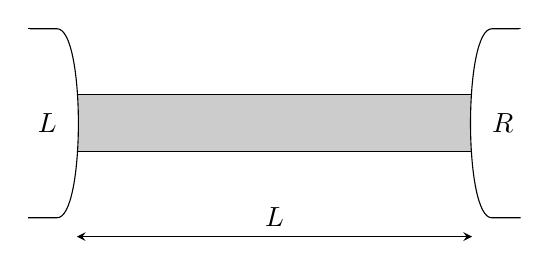
\begin{tikzpicture}[scale=1.2]
        %sistema mesoscopico
        \draw[fill=gray!40!] (-2.11,0.3) -- (2.11,0.3) -- (2.11,-0.3) -- (-2.11,-0.3) -- cycle;
        %Reservoir
        \draw[fill=white] (-2.6,-1) -- (-2.3,-1) .. controls (-2,-1) and (-2,1) .. (-2.3,1) -- (-2.6,1) -- cycle;
        \draw[white,thick,shorten <= 0.22pt,shorten >= 0.22pt] (-2.6,-1) -- (-2.6,1);
        \draw[fill=white] (2.6,-1) -- (2.3,-1) .. controls (2,-1) and (2,1) .. (2.3,1) -- (2.6,1) -- cycle;
        \draw[white,thick,shorten <= 0.22pt,shorten >= 0.22pt] (2.6,-1) -- (2.6,1);
        % Etichette nei contatti
        \node[left] at (-2.2,0) {$L$};
        \node[right] at (2.2,0) {$R$};
        % Distanza L con frecce
        \draw[stealth-stealth,shorten <= -0.11cm, shorten >= -0.11cm] (-2,-1.2) -- (2,-1.2) node[midway, above] {$L$};
    \end{tikzpicture}
\end{figure}
\hspace{-0.6cm}Per serbatoio ideale intendiamo che il numero di elettroni al suo interno è talmente elevato che la sua temperatura e il suo potenziale chimico restano invariati anche se un elettrone abbandona o entra nel reservoir, in quanto $N\approx N+1$ per $N$ grande.\\
Tale assunzione implica che quando il numero di elettroni del reservoir varia, questo ritorni istantaneamente ad uno stato di equilibrio, rendendo possibile descrivere gli elettroni dei reservoir mediante la distribuzione di Fermi-Dirac:
\begin{equation}
    f_D(E,\mu,T)
    = \frac{1}{\exp \bigl[ (E - \mu)/(k_B T) \bigr] + 1}
    \label{eq:distribuzione_Fermi-Dirac}
\end{equation}
Essa ci dà la frazione di elettroni aventi energia $E$ a temperatura $T$ e potenzialiìe chimico $\mu$ fissati.\\
Ricordiamo che tale distribuzione segue l'andamento riportato in figura:
\begin{figure}[H]
    \centering
    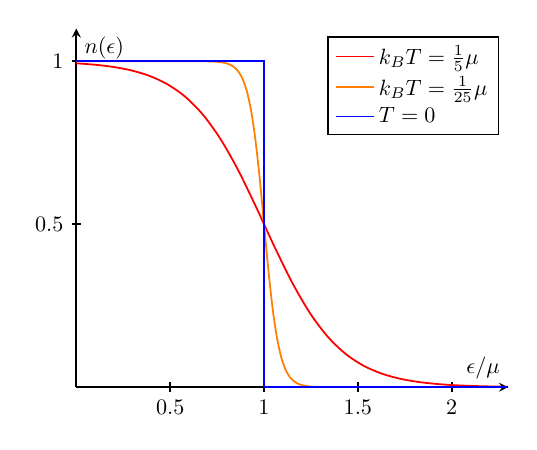
\begin{tikzpicture}[scale=.8]
        \begin{axis}[
            xlabel=$\epsilon/\mu$,
            ylabel=$n(\epsilon)$,
            domain=0:2.3,ymax=1.1,
            ytick={0.5,1},
            smooth,thick,
            axis lines=center,
            every tick/.style={thick},
            legend cell align=left]
      
          % Graphs
          \def\chempot{1}
          \def\n#1{1/(e^(#1*(x - \chempot)) + 1)}
          \addplot[color=red]{\n{5}};
          \addplot[color=orange,samples=100]{\n{25}};
          \addplot[const plot,color=blue] coordinates {(0,1) (\chempot,0) (2.3,0)};
      
          \legend{$k_\text{B} T = \frac{1}{5} \mu$,$k_\text{B} T = \frac{1}{25} \mu$,$T = 0$}.
        \end{axis}
      \end{tikzpicture}
\end{figure}
\textbf{DISEGNO PROVVISORIO}\\
Quando $T\to 0$, essa tende a una funzione a gradino, mentre a temperatura finita ha un andamento più smussato.\\
In generale, i due serbatoi possono avere temperature $T_L$ e $T_R$ o potenziali chimici $\mu_L$ e $\mu_R$ diversi. Il modo più semplice per avere, ad esempio, due potenziali chimici diversi è quello di applicare una differenza di potenziale tra i due serbatoi\mn{Se invece volessimo realizzare una differenza di temperatura è sufficiente applicare un gradiente termico.} collegandoli ad un generatore di tensione, il quale permetterà di modulare $\mu_L$ e $\mu_R$:
\begin{figure}[H]
    \centering
     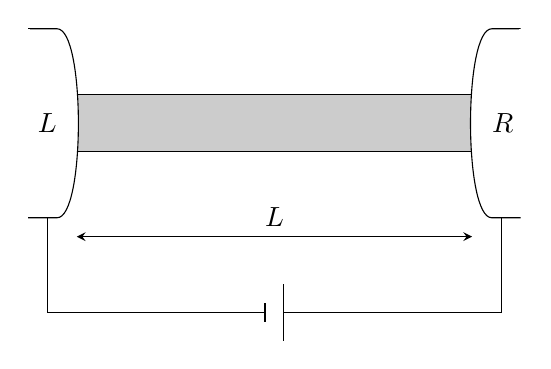
\begin{tikzpicture}[scale=1.2]
        %sistema mesoscopico
        \draw[fill=gray!40!] (-2.11,0.3) -- (2.11,0.3) -- (2.11,-0.3) -- (-2.11,-0.3) -- cycle;
        %Reservoir
        \draw[fill=white] (-2.6,-1) -- (-2.3,-1) .. controls (-2,-1) and (-2,1) .. (-2.3,1) -- (-2.6,1) -- cycle;
        \draw[white,thick,shorten <= 0.22pt,shorten >= 0.22pt] (-2.6,-1) -- (-2.6,1);
        \draw[fill=white] (2.6,-1) -- (2.3,-1) .. controls (2,-1) and (2,1) .. (2.3,1) -- (2.6,1) -- cycle;
        \draw[white,thick,shorten <= 0.22pt,shorten >= 0.22pt] (2.6,-1) -- (2.6,1);
        % Etichette nei contatti
        \node[left] at (-2.2,0) {$L$};
        \node[right] at (2.2,0) {$R$};
        % Distanza L con frecce
        \draw[stealth-stealth,shorten <= -0.11cm, shorten >= -0.11cm] (-2,-1.2) -- (2,-1.2) node[midway, above] {$L$};
        % circuito
        \draw (-2.4,-1) -- (-2.4,-2) -- (-0.1,-2);
        \draw[thick] (-0.1,-2.1) -- (-0.1,-1.9);
        \draw (0.1,-2.3) -- (0.1,-1.7);
        \draw (0.1,-2) -- (2.4,-2) -- (2.4,-1);
    \end{tikzpicture}
 \end{figure}
\hspace{-0.6cm}In conseguenza a tale differenza di potenziale chimico, si verificherà un flusso di elettroni tra i due reservoir, facendo comunque restare questi ultimi in equilibrio per le precedenti assunzioni.\\
(Di questo paragrafetto lascerei solo la prima nota, forse mettendola nella discussione sopra sui serbatoi ideali)Supponiamo che nei due serbatoi il sistema elettronico rimanga in equilibrio anche in presenza di una caduta di tensione o di una differenza di temperatura e, se vi è un flusso di corrente, assumiamo che nei due serbatoi avvenga un rilassamento istantaneo degli elettroni\sn{Per rilassamento istantaneo si intende un processo in cui un sistema passa da uno stato di non equilibrio a uno stato di equilibrio in un tempo trascurabilmente breve, praticamente istantaneo rispetto alle scale temporali del fenomeno in esame.}, i quali rimangono in equilibrio. Ciò significa che gli elettroni nei serbatoi possono essere sempre descritti dalla distribuzione di Fermi-Dirac, la quale rimane invariata\sn{Dubbio mio: ma visto che applichiamo il voltage drop non cambia il potenziale chimico? e quindi la distribuzione di Fermi-Dirac? probabilmente intende che la funzione di distribuzione è sempre una FD, come forma funzionale, ad un opportuno $\mu$}.\\
Studiamo il problema con una teoria semiclassica, dove con tale espressione intendiamo che nell'equazione che descrive il sistema figurano sia termini di tipo classico che altri di tipo quantistico. Più precisamente, descriviamo gli elettroni come particelle classiche e riteniamo la loro posizione e il loro impulso conoscibili contemporaneamente con precisione sufficientemente grande, figurando questi come variabili classiche in alcuni termini, mentre convenientemente come operatori quantistici in altri. Quantitativamente, ciò è ragionevole quando la lunghezza d'onda di Fermi, che rappresenta la larghezza del pacchetto d'onda e quindi l'incertezza sulla posizione della particella data dal principio di indeterminazione di Heisenberg, data da\sn{io ho trovato come def $\frac{2\pi}{k_F}=\frac{2\pi\hbar}{\sqrt{2m^*E_F}}$}
\begin{equation*}
    \lambda_F=\frac{\pi \hbar}{E_F},
\end{equation*}
essendo $E_F$ l'energia di Fermi, è molto più piccola di tutte le scale di lunghezza del sistema. Ciò significa che $\lambda_F$ deve essere molto più piccola delle dimensioni tipiche del sistema e dei diversi liberi cammini medi, cioè delle distanze percorse mediamente da un elettrone tra due eventi consecutivi di scattering della medesima tipologia. In particolare, nella nostra trattazione siamo interessati a tre tipi di liberi cammini medi:
\begin{itemize}[leftmargin=0.5cm]
    \item la lunghezza di scattering elastico $\ell_{\rm el}$, associata allo scattering degli elettroni con le impurità del sistema;
    \item la lunghezza di scattering elettrone-elettrone $\ell_{\rm e,e}$, legata allo scattering di elettroni con altri elettroni e dunque dovuta all'interazione coulombiana;
    \item la lunghezza di scattering elettrone-fonone $\ell_{\rm e,ph}$, associata allo scattering degli elettroni con i fononi del sistema.
\end{itemize}
Precisiamo i seguenti fatti:
\begin{itemize}[leftmargin=0.5cm]
    \item lo scattering tra elettroni e impurità è elastico, per cui l'energia dell'elettrone si conserva;
    \item lo scattering elettrone-elettrone non conserva l'energia del singolo elettrone ma l'energia totale dei due elettroni. Ciò è dovuto al fatto che nello scattering i due elettroni possono scambiare energia, come possiamo vedere nel seguente diagramma:
    \begin{figure}[H]
        \centering
        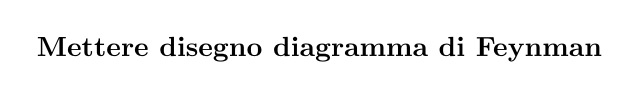
\begin{tikzpicture}
            \node at (0,0) {\textbf{Mettere disegno diagramma di Feynman}};
        \end{tikzpicture}
    \end{figure}
    Per quanto detto avremo che, se $E_1$ ed $E_2$ sono le energie prima dello scattering e $E_1'$ ed $E_2'$ le energie dopo lo scattering, allora avremo che in generale $E_1 \neq E_1'$ e $E_2 \neq E_2'$ ma $E_1 + E_2 = E_1' + E_2'$;
    \item nello scattering elettrone-fonone, in cui si ha l'assorbimento o l'emissione di un fonone di energia $\hbar \omega$, l'energia non si conserva, in quanto dopo lo scattering l'elettrone inizialmente avente energia $E$ avrà energia $E \pm \hbar \omega$, come possiamo vedere nei seguenti diagrammi:
    \begin{figure}[H]
        \centering
        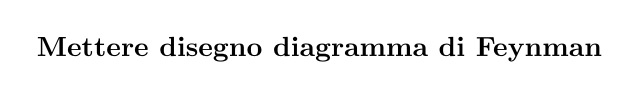
\begin{tikzpicture}
            \node at (0,0) {\textbf{Mettere disegno diagramma di Feynman}};
        \end{tikzpicture}
    \end{figure}
\end{itemize}
(Questo paragrafetto potrebbe essere da rivedere)A seguito di questi processi di scattering, se essi sono abbastanza efficienti, si ha un "dephasing", ossia una randomizzazione della fase della funzione d'onda. In conseguenza a ciò vengono meno tutti i processi coerenti come i processi di interferenza. Nel momento in cui vengono meno questi ultimi, la particella, a meno di correzioni di cui terremo conto, si comporta come una particella classica. Questo tipo di descrizione è tipico della fisica dei semiconduttori. Bisogna però stare attenti a che processo si sta studiando: ad esempio, tale approccio non funziona per studiare l'assorbimento inter-banda in cui vogliamo studiare il passaggio di un elettrone dalla banda di valenza alla banda di conduzione, in quanto il concetto di banda non esiste classicamente; al contrario, tale approccio funziona quando studiamo trasporto in corrente continua o modulato debolmente.\\
Ritornando al nostro sistema mesoscopico collegato ai due serbatoi, ci proponiamo di trovare la funzione di distribuzione degli elettroni in tale sistema.\\
Cerchiamo quindi una funzione\sn{Notiamo che la validità del concetto di funzione di distribuzione $f(\vb{r}, \vb{p},t)$ poggia sull'assunzione fatta precedentemente su $\lambda_F$.} $f(\vb{r},\vb{p},t)$ tale che la quantità
\begin{equation*}
    f(\vb{r},\vb{p},t) \frac{\dd[3]{\vb{r}} \dd[3]{\vb{p}}}{(2 \pi \hbar)^3},
\end{equation*}
cioè il prodotto tra essa e il volume elementare dello spazio delle fasi, ci dia la frazione di elettroni aventi posizione tra $\vb{r}$ e $\dd[3]{\vb{r}}$ e impulso tra $\vb{p}$ e $\dd[3]{\vb{p}}$ (la normalizzazione è fissata a 1 oppure a $g_S$?).\\
Per trovare la funzione di distribuzione ne studiamo l'evoluzione temporale. Dopo un tempo $\dd{t}$, la funzione di distribuzione sarà $f(\vb{r} + \vb{v} \dd{t}, \vb{p} + \vb{F} \dd{t}, t + \dd{t})$, dove $\vb{v}$ è la velocità dell'elettrone e $\vb{F}$ è la forza che agisce su di esso, generata dal campo elettromagnetico dovuto alla caduta di potenziale
%che assumiamo una dipendenza spaziale regolare
. Se non avvengono fenomeni di scattering, per il teorema di Liouville\mn{Esso afferma che un volumetto $\dd[3]\vb{r}\dd[3]\vb{p}$ dello spazio delle fasi centrato in $(\vb{r},\vb{p})$ evolve nello spazio delle fasi rimanendo invariato.(da sistemare)} la funzione di distribuzione rimane costante, ossia
\begin{equation*}
    f(\vb{r} + \vb{v} \dd{t}, \vb{p} + \vb{F} \dd{t}, t + \dd{t}) - f(\vb{r}, \vb{p}, t)
    =0
\end{equation*}
Se invece avvengono fenomeni di scattering, la funzione di distribuzione varia. Denotata con $I_{\rm coll}[f] \dd{t}$ tale differenza, dove $I_{\rm coll}[f]$ è detto integrale collisionale e tiene conto di tutti i processi di scattering, abbiamo che
\begin{equation}
    f(\vb{r} + \vb{v} \dd{t}, \vb{p} + \vb{F} \dd{t}, t + \dd{t}) - f(\vb{r}, \vb{p}, t)
    =I_{\rm coll}[f] \dd{t}
    \label{eq:differenza_funzione_distribuzione_con_collisioni}
\end{equation}
Il membro destro dell'Equazione \eqref{eq:differenza_funzione_distribuzione_con_collisioni} rappresenta il termine quantistico nell'equazione che descrive il nostro sistema.\\
Consideriamo il membro di sinistra ed espandiamo al primo in ordine in $\dd{t}$, ottenendo\sn{da fare il comando smallo per fare opiccolo calligrafico.}
\begin{equation*}
    \begin{split}
        & \hspace{0.1cm} f(\vb{r} + \vb{v} \dd{t}, \vb{p} + \vb{F} \dd{t}, t + \dd{t}) - f(\vb{r}, \vb{p}, t)
        \\
        = & \hspace{0.1cm} f(\vb{r}, \vb{p}, t) + \pdv{f}{\vb{r}} \vdot \vb{v} \dd{t} + \pdv{f}{\vb{p}} \vdot \vb{F} \dd{t} + \pdv{f}{t} \dd{t} - f(\vb{r}, \vb{p}, t) +o{(\dd{t})^2}
        \\
        \approx & \hspace{0.1cm} \pdv{f}{\vb{r}} \vdot \vb{v} \dd{t} + \pdv{f}{\vb{p}} \vdot \vb{F} \dd{t} + \pdv{f}{t} \dd{t}
    \end{split}
\end{equation*}
Utilizzando quanto trovato, otteniamo
\begin{equation}
    \pdv{f}{\vb{r}} \vdot \vb{v} + \pdv{f}{\vb{p}} \vdot \vb{F} + \pdv{f}{t}
    =I_{\rm coll}[f],
    \label{eq:equazione_di_Boltzmann}
\end{equation}
che è chiamata equazione di Boltzmann.\\
Puntualizziamo che in assenza del termine collisionale, l'equazione di Boltzmann prende il nome di equazione di Vlasov:
\begin{equation}
    \pdv{f}{\vb{r}} \vdot \vb{v} + \pdv{f}{\vb{p}} \vdot \vb{F} + \pdv{f}{t}
    =0.
    \label{eq:equazione_di_Vlasov}
\end{equation}
(paragrafetto da sistemare spiegando meglio che nel sistema i cammini liberi medi e $\lambda_F$ devono essere in relazione tale che $\lambda_F$ deve essere molto più piccola dei liberi cammini medi ma questi devono essere abbastanza piccoli e quindi i processi di scattering abbastanza efficienti da randomizzare la fase della funzione d'onda e poter trascurare processi coerenti)Quindi, quando i processi di scattering sono trascurabili e dunque il sistema si comporta in maniera pulita ma lo possiamo ancora trattare semiclassicamente. Si presti attenzione al fatto che tale fatto non è per niente banale, in quanto come abbiamo detto se un sistema è pulito vuol dire che sono trascurabili i processi di scattering, ma ciò implica che probabilmente si verificano processi coerenti, quindi fenomeni di interferenza quantistica, per non potremmo utilizzare questa trattazione. In ultima analisi, le situazioni in cui è possibile utilizzare l'\eqrefcustom{eq:equazione_di_Vlasov} sono poche.\\
Torniamo adesso all'\eqref{eq:equazione_di_Boltzmann}. E' utile esprimere la dipendenza da $\vb{p}$ tramite le coordinate sferiche, dunque dividendo la dipendenza dalla parte angolare da quella radiale. In tali termini, la funzione di distrubizione sarà nella forma $f(\vb{r},\vu{p},E)$, dove abbiamo messo l'energia al posto del modulo $p$ perché la relazione di dispersione è del tipo
\begin{equation*}
    \varepsilon(\vb{p})=
    \frac{\vb{p}^2}{2m}
\end{equation*}
dove $m$ è la massa efficace dell'elettrone\mn{Infatti stiamo usando implicitamente l'approssimazione di elettroni liberi.}.\\
In tale forma, il termine contenente la derivata rispetto a $\vb{p}$ nell'\eqrefcustom{eq:equazione_di_Boltzmann} diventa
\begin{equation*}
    \pdv{f}{\vb{p}} \vdot \vb{F}
    =\pdv{f}{\vu{p}} \pdv{\vu{p}}{\vb{p}} \vdot \vb{F} + \pdv{f}{E} \pdv{E}{\vb{p}}\vdot \vb{F} 
\end{equation*}
Tuttavia, il primo termine del membro di destra risulta essere trascurabile, vedremo a breve perché.\\
Possiamo quindi scrivere
\begin{equation*}
    \pdv{f}{\vb{p}} \vdot \vb{F}
    =\pdv{f}{E} \pdv{E}{\vb{p}}\vdot \vb{F}
\end{equation*}
D'altra parte, il gradiente della relazione di dispersione rispetto all'impulso $\vb{p}$ non è altro che la velocità di gruppo $\vb{v}$,\mn{Infatti, esplicitamente si ha
\begin{equation*}
    \grad_{\vb{p}} \varepsilon(\vb{p})
    =\grad_{\vb{p}} \frac{\vb{p}^2}{2m}
    =\frac{\vb{p}}{m}
    \equiv \vb{v}
\end{equation*}} per cui in definitiva abbiamo che
\begin{equation*}
    \pdv{f}{\vb{p}} \vdot \vb{F}
    =\pdv{f}{E} \vb{v} \vdot \vb{F}
\end{equation*}
Supponiamo adesso che la forza sia dovuta soltanto al campo elettrico, dunque sia nella forma $\vb{F}=q\vb{E}$ dove $q$ è la carica. Allora, ricordando che $\vb{E}=-\partial_{\vb{r}} \phi$, per quanto detto il termine dell'\eqref{eq:equazione_di_Boltzmann} contenente $\vb{F}$ diventa
\begin{equation*}
    \pdv{f}{\vb{p}} \vdot \vb{F}
    =\pdv{f}{E} \vb{v} \vdot \qty( -q \pdv{\phi}{\vb{r}} )
    =\pdv{f}{E} \qty( -q \pdv{\phi}{\vb{r}} ) \vdot \vb{v}
\end{equation*}
e dunque possiamo riscrivere l'\eqrefcustom{eq:equazione_di_Boltzmann} come
\begin{equation*}
    \pdv{f}{\vb{r}} \vdot \vb{v} + \pdv{f}{E} \qty( -q \pdv{\phi}{\vb{r}} ) \vdot \vb{v} + \pdv{f}{t}
    =I_{\rm coll}[f]
\end{equation*}
ovvero, raggruppando i termini,
\begin{equation}
    \qty( \pdv{f}{\vb{r}} - q \pdv{\phi}{\vb{r}} \pdv{f}{E} ) \vdot \vb{v} + \pdv{f}{t}
    =I_{\rm coll}[f]
    \label{eq:equazione_di_Boltzmann_con_campo}
\end{equation}
Se inglobiamo nell'energia la dipendenza del potenziale dalla posizione, il che corrisponde a dire che $f$ ha una dipendenza del tipo $f(\vb{r},\vb{p}, E - q \phi(\vb{r}))$, il termine tra parentesi della \eqref{eq:equazione_di_Boltzmann_con_campo} diventa proprio $\pdv*{f}{\vb{r}}$, per cui possiamo scrivere più sinteticamente
\begin{equation}
    \pdv{f}{\vb{r}} \vdot \vb{v} + \pdv{f}{t}
    =I_{\rm coll}[f]
    \label{eq:equazione_di_Boltzmann_con_campo_sintetica}
\end{equation}
Osserviamo che se $f(\vb{r},\vb{p}, E - q \phi(\vb{r}))$ si comportasse come una funzione di distribuzione di Fermi-Dirac, ciò significherebbe che nell'\eqrefcustom{eq:distribuzione_Fermi-Dirac} al posto di $\mu$ dovremmo scrivere $\mu + q\phi(\vb{r})$, cioè è come se ci ritrovassimo un potenziale chimico che dipende dalla posizione. Come vedremo, quando $f$ prende la forma di una funziona di Fermi-Dirac efficace, tale $\mu$ prenderà il nome di potenziale elettrochimico.\\
Prima di proseguire, facciamo una stima dell'ordine del termine relativo alla derivata rispetto a $\vu{p}$ che abbiamo trascurato, in modo da capire quanto è grande l'errore che commettiamo nel trascurarlo. Osserviamo che $\pdv*{f}{\vu{p}}$ è adimensionale perché $f$ è una densità di probabilità, dunque possiamo concentrarci sulla parte $\pdv*{\vu{p}}{\vb{p}} \vdot \vb{F}$: nella parte $\pdv*{\vu{p}}{\vb{p}}$, $\vu{p}$ non ha dimensioni, mentre $\vb{p}$ ha le dimensioni di un impulso ed in particolare è dell'ordine dell'impulso di Fermi $p_F$; $F$ invece è una forza elettrica che è dell'ordine della carica moltiplicata per la differenza di tensione applicata divisa la lunghezza del campione. In definitiva abbiamo:
\begin{equation*}
    \qty[ \pdv{f}{\vu{p}} \pdv{\vu{p}}{\vb{p}} \vdot \vb{F} ]
    \sim \frac{1}{p_F} \frac{qV}{L}
\end{equation*}
Moltiplicando e dividendo per $\frac{p_F}{m}$ otteniamo
\begin{equation*}
    \frac{1}{p_F} \frac{qV}{L}
    =\frac{1}{p_F} \frac{qV}{L} \frac{p_F}{m} \frac{m}{p_F}
    =qV \frac{m}{p_F^2} \frac{1}{L} \frac{p_F}{m}
\end{equation*}
Notiamo che $m/p_F^2$ è dell'ordine dell'inverso dell'energia di Fermi, ossia $1/E_F$, mentre $p_F/m$ è dell'ordine della velocità di Fermi $v_F$. In definitiva otteniamo
\begin{equation*}
    \frac{1}{p_F} \frac{qV}{L}
    \sim \frac{qV}{E_F} \frac{v_F}{L}
\end{equation*}
Il termine $v_F/L$ rappresenta la scala dell'inverso dei tempi tipici dell'\eqrefcustom{eq:equazione_di_Boltzmann_con_campo_sintetica}, dunque per capire se tale termine è trascurabile dobbiamo guardare l'ordine di grandezza di $qV/E_F$. In un conduttore, l'energia di Fermi è tipicamente dell'ordine dell'eV o di frazioni dell'eV, mentre $qV$ in genere è dell'ordine dei $\rm \mu eV$, dunque tale termine risulta essere dell'ordine di $10^{-6}$, per cui è lecito trascurarlo. Precisiamo che omettere tale termine equivale sostanzialmente a trascurare il disturbo nella parte angolare della funzione di distribuzione dovuto a una tensione o ad un gradiente termico.
\begin{example}[Equazione di Boltzmann per un filo ballistico.]
    Consideriamo un filo quasi-unidimensionale come quello riportato nella figura seguente:\mn{Disegno da fare il Latex, ora mi secco.}
    \begin{figure}[H]
        \centering
        \includegraphics[width=0.7\textwidth]{Immagini/Ballistic_wire.png}
    \end{figure}
    Diciamo che tale sistema è quasi-unidimensionale perché supponiamo che l'ampiezza $W$ del filo sia molto minore della lunghezza $L$ del filo stesso.\\
    Supponiamo che non contenga impurità, sia perfettamente rettangolare e abbia bordi regolari, in modo che risulti $I_{\rm coll}[f]=0$. Nel limite statico, in cui $\partial_t f=0$, l'\eqrefcustom{eq:equazione_di_Boltzmann} assumerà allora forma
    \begin{equation*}
        \vb{v} \vdot \grad_{\vb{r}} f(\vb{r},\vu{p},E)
        =0
    \end{equation*}
    Supponendo che i serbatoi sinistro e destro seguano rispettivamente dele distribuzioni di Fermi-Dirac $f_L(E)$ ed $f_R(E)$, la funzione di distribuzione sarà data da:
    \begin{equation*}
        f(\vb{r},\vu{p},E)
        =
        \begin{cases}
            f_L(E) & \text{se } \vu{p}_x<0 \\
            f_R(E) & \text{se } \vu{p}_x>0
        \end{cases}
    \end{equation*}
    Il risultato trovato ci dice che, in assenza di collisioni, i due serbatoi restano indipendenti; inoltre gli elettroni iniettati da sinistra seguono la funzione di distribuzione del serbatoio sinistro anche nel sistema mesoscopico (cioè dentro il cavo) e gli elettroni iniettati da destra nel sistema avranno la funzione di distribuzione del serbatoio destro.\mn{Così come riportato in \cite{Heikkila}, ciò significa che "Il sistema di elettroni all'interno del filo è quindi composto da elettroni che si muovono verso sinistra e elettroni che si muovono verso destra, che non si mescolano in assenza di diffusione e che sono distribuiti in energia secondo le funzioni di distribuzione nei serbatoi da cui provengono."}
\end{example}
\section{Osservabili}
Il motivo per cui siamo interessati a trovare la funzione di distribuzione è che possiamo esprimere le osservabili del sistema in termini di essa. In particolare, la densità di portatori di carica del sistema sarà data da\mn{Infatti integrando $f$ rispetto all'impulso otteniamo la densità di probabilità di trovare un elettrone in posizione $\vb{r}$, cioè proprio la densità di portatori.}
\begin{equation*}
    n(\vb{r})
    =g_s \int \frac{\dd[3]{\vb{p}}}{(2 \pi \hbar)^3} f(\vb{r},\vb{p},t)
\end{equation*}
dove $g_s$ è la degenerazione di spin, che nel caso in esame è semplicemente pari a 2.\\
Analogamente, la densità di corrente sarà data da\mn{Abbiamo scritto la velocità come $\vb{v(p)}$ per sottolineare che essa è data da $\grad_p \varepsilon(\vb{p})$.}
\begin{equation*}
    \vb{j}_c(\vb{r})
    =-e g_s \int \frac{\dd[3]{\vb{p}}}{(2 \pi \hbar)^3} \vb{v}(\vb{p}) f(\vb{r},\vb{p})
\end{equation*}
Passando in coordinate polari possiamo riscrivere tale quantità come
\begin{equation*}
    \vb{j}_c(\vb{r})
    =-e g_s \int \dd{p} p^2 \int \frac{\dd{\vu{p}}}{(2\pi\hbar)^3} \vb{v}(\vb{p}) f(\vb{r},\vu{p})
\end{equation*}
dove l'integrazione rispetto a $\vu{p}$ è esplicitamente data da
\begin{equation*}
    \int \dd{\vu{p}}
    =\int_{0}^{2\pi} \dd{\varphi} \int_{0}^{\pi} \dd{\vartheta} \sin{\vartheta}
\end{equation*}
Se adesso esprimiamo $p^2$ come $p^2=2mE$, da cui segue che $2p \dd{p}=2m \dd{E}$, abbiamo che
\begin{equation*}
    \dd{p} p^2
    =\sqrt{2} m^{\frac{3}{2}} \sqrt{E} \dd{E}
\end{equation*}
e inoltre possiamo riscrivere $\vb{j}_c$ come
\begin{equation*}
    \vb{j}_c(\vb{r})
    =-e \int \dd{E} N(E) \int \frac{\dd{\vu{p}}}{4\pi} \vb{v}(\vb{p}) f(\vb{r},\vu{p})
\end{equation*}
dove
\begin{equation*}
    N(E)
    =\frac{\sqrt{2E} m^{\frac{3}{2}}}{\pi^2 \hbar^3}
\end{equation*}
è la densità degli stati di una particella libera in un sistema tridimensionale.\\
\textbf{1:00:15 circa}
%che ha una dipendenza dall'energia a radici. Però non si separava la despicità di tendenza angolare, di solito il fatto che l'energia di un tesoro dal modulo si cambiava la gaffa di gaffa. Perché la partangolare è da se mangiata quando fai il genico, questo come comunque non sai qua che succederà, che da dividere in ghiaccio in altri. Se esistisci questo conto in 2D come va a reprendere gli stati, flat, solamente. Se la faccio in 1D come direi le densità degli stati di raggiungere. Quindi in 2D a meno di questo 3D, se li facesti la stessa cosa, immaginando un sistema 2D, la densità degli stati se parte più che lo su 2M viene una costante. Se la faccio invece in 3D, mi viene una roba di questo tipo che è una divergenza integrabile. La differenza della densità registra di le fattore singuramente divano, sono solide. Tutte divergenze integrabili, perché se hai preso un conto e provate una divergenza di un'insidestra che non è integrabile, hai risposto. Perché il flat da c'è, non è possibile che da una cosa in cui contate gli stati viene vengono più, non mi corrisponde una cosa che non è contabile, perché se le partite da una cosa che è integrabile, hai fatto soltanto un cambiamento di variabili per coppare la fittura. Questo è un miscule che dice che c'è in Eh, non è zero, dire che è costante. Ok, grazie. Cos'è che voglio dire con questa cosa? Allora, questa cosa che è la divergenza in 1D, va come una cadice, capite subito che i sistemi 1D sono un po' più speciali, c'è un po' di caratteristiche per cui non è solo questo che me lo dice, ma i sistemi 1D sono quei sistemi in cui non funziona, quella che viene che chiamarsi teoria di Landau, dei periodi di fermi. Cioè, non l'avete fatto in molti coppi, molti coppi, ma anche Cioè, è stato tonico. Cioè, il fatto è che io ho un sistema fortemente intelligente, e poi dopo tutto il suo casino ci metto tutte le azioni, termini di scambio con le azioni, i carti, i foc, i bubpet, e alla fine questa cosa che mi fa, oh, un'ettronome che camina là dentro, ecco, questa cosa che io descrivo, un sistema fortemente un sistema intelligente, come una particella, con una certa carica, con una certa codizione, è possibile, nei sistemi equivale, quelle che si chiano teoria teoria degli teoria delle alibi dei fermi, possia il fatto che posso descrivere il mio sistema elettronico come una quasi particella con le proprietà tipiche della particella dell'elettrolem, ma tutte rinnovoliziate. Se cosa funziona, per esempio, un unutto 3D, un unutto 2D, ma già in un unutto 1D non funziona più. Perché inizia a partire a un certo punto in ridi per gente, e per cui questo tipo di rinnovolizia non lo può fare più. Solo so, vi dico, perché se a me lo si semplice, secondo me, diplicamente, non ho tutto, è un'ottima di sicursa, per esempio, che si chiamano teoria di Latinge, che ha una teoria multicorpia, che non ha nulla, che può vedere quel mondo classico. Io lo sto dicendo, è un'ottima di certo. Sesso, non era solo per mi ha detto che niente. No, così no, questo è un'ottima di certo. Questo è, ma la teoria di un unutto L'atinge, ha scritto l'utting. L'altra cosa che volevo fare, portare questa cosa da da vecchio con buone, in questo modo di rinnovolizia, è che, allora, in questa cosa, ha l'inserio costante.
Graficamente il comportamento di $N(E)$ in funzione dell'energia è il seguente:
\begin{figure}[H]
    \centering
    \begin{tikzpicture}[scale=1.2]
        \draw[->] (0,0) -- (5,0) node[right] {$E$};
        \draw[->] (0,0) -- (0,2.5) node[above] {$N(E)$};
        \draw[dashed] (4,0) node[below] {$E_F$} -- (4,2);
        \draw[thick, teal!50!green] plot[smooth, domain=0:5,samples=400] (\x, {sqrt(\x)});
    \end{tikzpicture}
\end{figure}
\hspace{-0.6cm}Dal grafico si evince che, se operiamo in una finestra di energia attorno all'energia di Fermi spostandoci da essa al massimo di una quantità $\pm kB T$, poiché l'energia di Fermi è dell'ordine della frazione di eV, mentre la temperatura ambiente (cioè circa $300 \; \rm K$) corrisponde a $25 \; \rm meV$, è lecito trattare la densità degli stati come approssimativamente costante.\mn{Da ora in poi, tratteremo la densità degli stati come costante. Quando non sarà possibile fare ciò lo specificheremo.}
\section{Approssimazione di tempo di rilassamento}
%Quindi, l'idea è questa, ora lo siano una scheme per approcciare l'intero colisione e scrivere l'intero colisione in termini di tempo di relazione. Quindi, cosa è la relazione? Ho la funzione di distribuzione, quindi la funzione di distribuzione di andare, e lo descrive, che è l'inglese di numero in questo spazio in il mio sistema. E, se il mio sistema è un equilibrio, f è uguale a una f0, f0 è il mio equilibrio di distribuzione. Se colgo il mio sistema è un equilibrio, in questo caso, di gramma che ho rubato Per fare questa lezione, ho scippato un pezzo di ramerd dalle ferrovie e ce l'ho messo così da solo da una persona del ligno, a temperatura esattima, a l'ambiente, potenziale chimico, quello tuo, che c'ha indrincegamente una certa concentrazione di elettrono, che può fare potenziale chimico, un seguito. Se lo connetto, per esempio, a attenzione, oppure, in mezzo a due o due un controllo di lindere, è un libro che si è una diverse. Quindi, c'è la modula, e, tanto io, la diversione rispetto all'equilibrio, o che l'equilibrio è l'F. Se, per l'esercito di l'esercito questa settimana, l'F è molto più piccola che l'F, non è. Tee, per esempio, la collisione interna è un funzione di funzione di distribuzione, di l'F può essere approximata con E e 0 plus l'E l'F dove F è anche in F, non l'E quindi, io linearizzo quindi, tipicamente, l'E collisione interna è una dependenza non limitata di la distribuzione ma se l'E è una più quantità io linearizzo l'E collisione interna con l'esercito di l'equilibrio di distribuzione, funzione e questa è la distribuzione che è questo scale di questo derivativo quindi, se osservo la questione di both, ho l'E T plus B H F l'E dà l'E faccio tipo l'equazione l'homogerità dell'equazione per controllare F è un numero pure questa è la derivazione che ti aspettavo quindi, qua mi devi regalare l'E di conseguenza, questo è il suo inverso questo è il suo inverso che è la derivata del collisionale e la derivata la iniziale, distribuzione e adesso non dà questi tempi sono appunto i tempi di scattere in un definito e in particolar io avrei un po' di questo minus di over ok e noi abbiamo un tau per ogni classe di collisioni quindi se ho un elettro iniziale scattere ho un scattere due a elastica scattere con l'impurità se ho un elettro iniziale ho un scattere per l'energia scattere e ho un elastico e t se fì, è un scattere elettro ok, tipicamente io posso usare per comparare questo scattere posso usare ogni momento o moltiplare per la velocità termina e per moltiplare per la velocità termina t, l, ho l'alto scattere o è il stesso perché il tau è il tempo tra due elettro iniziale scattere ma se la velocità tipica dell'elettro è la velocità termina il length tra le elettro iniziale è il motivallare del tau è un motivallare di un minuto iniziale niente e androggendo dalla modalità fisica ok per la comparazione di questo length scale l, l l, e, e e l, e, e io ho un tipo di tritura di tritura di tritura di tritura quindi c'è un po' di inomenzatura o di esologi quindi il santo del mio sistema è molto smaller di , e quindi il santo è molto smaller di tutte le scattere quindi mi significa che il mio elettro può trasferire l'entire sistema senza scattere perché se la lunghezza è più piccola di questo lui parte per il mangue tempo ah ma sono rilasco ok questo regime è il regime palese ok ma se con l, e, l questo è molto smaller il length del mio sistema quindi per esempio ok in questo caso questo è il regime diffusivo il regime diffusivo ok il regime diffusivo il più importante scattere il processo è di elettro e neggiore di scattere e questo è il tipico regime di transport in condizioni al semi-condatto cioè se voi fate un'invenzione in un pm, in un in cosa che volete di siciccio assenare un rigaggio quello che volete è lavorare a temperatura sufficientemente elevata in un elevato d'intento in un motore ambiente sostanzialmente il transport è del tipo diffusivo quindi in maniera grezza sostanzialmente è quello che descrittedemi della terria di Dure cioè capito in soquare non so c'è proprio base, base ma quasi però dico già quello che scrive abbastanza bene quello che succederà ok so, if the much smaller scatting length is the electron length of scattering in this case this regime is quasi equilibrating and we will verify that in this case the distribution function in my system is effectively expressed in this form ok so this is the distribution function in my system and I will have no no no no no no no no no no no ok in my system ok, direllamente devo cercare la funghi di distribuzione se io sono in questo regime in cui la la lunghezza più piccola è sempre la più importante perché significa che perché se la lunghezza è più piccola più piccola po' di muove e poi un po' di scatting e poi siamo attumbolate da l'interazione quindi è un'interazione in prinsa infatti questo, di regime qualcuno lo può avere in sistemi che hanno una mobilità infatti c'è la preferenza oppure l'assimilio di gallio in regime quello che si chiama the lesion doving l'accio un attimo di gallio un attimo leion doving è un tipo di tecnica in cui si faranno nelle quanti un bel, in nessuno di gallio che ha permesso per la prima volta di vedere l'effetto d'indistica in cui c'è una diverse andata del colore di questo sistema allora in questi sistemi come questa è in prinsa? devo dire che i processi di scatting stem, sistema elettronico sono meno efficaci di quello in cui si chiama quello che succede è che la tonia di distribuzione, magicamente ha la forma di una funzione di distribuzione di equilibrio ma non è di equilibrio perché ha una dipendenza della potenziale chimica della temperatura che dipende dalla potenziale chimica e sta cosa nel senso perché all'equilibrio del modinamico, temperatura della potenziale chimica non deve dipende dalla potenziale chimica cioè sì, la nonna dice cacce friddo cacce capro però la mia nonna, la mia nonna è in quasi equilibrio però cosa significa però efficaciamente quello che succede è che io per esempio ogni sistema so qua è mio sistema è che c'è una regione in cui posso descrivere inghezza tipicamente dell'ordine di L e E dove il sistema si comporta all'equilibrio ma per comportarsi all'equilibrio significa che ci deve essere qualcosa che lo termalizza cioè per termalizzare che significa che serve qualche processo fortemente non lineare che mi porti in un sistema ah diciamo da 3,0 alla più bassa inizia cioè se io un sistema lo faccio in maniera grezza grezza in senso un po' di figura avrebbe attorga cioè questo elettrone che viene ad altissima energia lanciava un reservoir dentro il suo sistema il mio sistema che mi scrivendo se io non ho nessun processo di termalizzazione quello che si chiama elettrone caldo parte questa questa energia deve essere messa in questo modo questa energia è più unito quello che succede se l'interazione dell'elettrone dell'elettrone è abbastanza importante che gli elettroni che in tempo basse energia fanno fare x-ter dopo vengono a prendere colpi di scattering e si distribuiscono tra di loro l'energia lui termalizza e a basse di energia dando una cotteia e il sistema ritorna a stanzialmente alle tecniche quello che succede questa questa è una raccuna l'elettrone sta bullizzata quindi quello che succede è che però questo processo cioè se sono una situazione di realtà fuori equilibrio di questa cosa e che localmente il sistema si comporta da un sottosto dell'equilibrio ma globalmente il sistema non è almeno quindi quello che si avrà è quello che si si avrà un gradiente di temperatura cioè proprio che lo posso seguire o un gradiente di potenziale chimico che significa che la concentrazione dell'elettrone può cambiare nella posizione infine l'altro regime potrebbe essere anche quello che è l'elettrone che fa un scattering è più importante quindi più per equilibrio allora in questo caso parlo di local equilibrio ok in local equilibrio FD è espressa E M R T ok è molto simile per questo ma qui ho un potenziale chimico che dipende della posizione ma quella temperatura è consente che è questa temperatura è quella della temperatura quindi in questo senso ok, ho le mie elettroni qui le mie elettroni stanno in un cristal stanno in un in stanno in un cristal e i fondamenti sono in equilibrio i fondamenti sono in equilibrio e perché per elettrone il elettrone è in una temperatura di la stessa cioè sostanzialmente quella cosa che vi ho raccontato prima che gli elettroni puliziano per il simbolo del trone che veniva iniettato lo fanno anche i voloni cioè se io il mio cristallo con i fondamenti è dei fondamenti che sto parlando lo fanno di volone, cristallo cioè il sonnado come se l'endampus sono le vibrazioni pedicolari regime quantissime sono le situazioni di vibrazioni pedicolari il corrispettivo del fotone del campo elettromagnetico in un cristallo diciamo i giovani che possono vibrare i regimi quantissimi che stanno in un fondamenti e sono dei bosoni hanno una funzione di distribuzione di tipo bosenister che laterizzate 

%un potenzio elichimico in realtà è una cosa di fondamenti in caso di elichimico è inizio a zero perché pensi con zero e la temperatura è la temperatura del tempio quello che abbiamo la temperatura del tempio insieme degli elettroni molto caldi e i fondamenti cioè che salo più freddo quello che succede che i fondamenti iniziano a prendere in realtà quello che succede che l'elettrono molto caldo che fa iniziare a mettere tanti fondamenti fin quando perde infatti tipicamente la temperatura del sistema elettronico è la stessa cosa può succedere io dico di ingetti i regimi e questa cosa penso che la farà a tono di inero così in genere che si può, per esempio se io prendo un lase nel pulsato posso prendere gli elettroni e farlo isolare nell'energia e c'è un talcente in cui il cristallo è che so vendi kevin e gli elettroni si ritrovano a migliaia che c'è un lato poi termalizzano e si ritrovano lo stesso dentro domande questa fase quindi di equilibrio locale soltanto termino, non chimico ad esempio in che systemi si trova tipicamente in realtà c'è quello sopra quindi il equilibrio locale termino e chimico ad esempio al dettono e il graffene si però dico nel caso in cui tu azzi a te un certo in genere se la temperatura delle barbine in sé è un po' più grande questo è questo, più o meno se io sono in un sistema molto pulito quindi ti miglia che mi posso per un attimo dimenticare delle impurezza allora se mi ritrovo la temperatura a bassanza bassa ma non troppo ora scrivo che è il mio graffene 200 kevin per uno che fa da sport di caldo 100-200 kevin allora in quel caso in media fa noni tempi e cenepochini e quindi fa in modo questo regime che lo scatte in elettrono e elettrono il più efficiente e quindi io trovo uno stricce nemmeno se io alzo la temperatura i fononi iniziano a crescere il numero di fononi perché quelli termici vanno iniziano a crescere con la temperatura e quindi lo scatte in elettrono e fonone anche se che la prende la lunghezza di scatte in elettrono e fonone che dipende da due cose dalla matrice di scatte ma dal numero di fononi se io ho una matrice di scatte invece la probabilità di scatte in elettrono ma poi ho 10 miliardi di fononi inizia a sennobbortare allora in quel caso se io ho un momento la temperatura mi ritrovo quindi il sistema mi ritroverò con una temperatura che è sostanzialmente quella del il numero di fononi come posso fare a fare in modo che questa cosa viene soppressa c'è a via o a via o a via o a via o a via o a via o a o o a via a a via a a via a come farebbe il teorico no che io sono qui da più che non è idea perché non so come si fa però faccioci mettiamo un criostrato e magari lo sperimentare e mi dici che stè ma c'è un altro problema di tecnologico che è un interessante allora mettono un gereno un criostrato e tengamo bassa la temperatura della questa perché dicevo non deve essere troppo basso perché se tu inizia da passare troppo la temperatura ah beh abbiamo capito la parte con i fononi perché è croda perché se ci sono coglifononi in giro non è una cosa che puoi fare qualche missione spondane cioè puoi fare qualche missione spondane un po' è piccolo proprio potresti fare scattere in attrione il corpo del principio e discusione di Paoli quello che succede è che se la temperatura è troppo bassa io non riesco a fare scattere in attrione in attrione e inizio dal principio di discusione di Paoli questo perché perché praticamente quando tu fai scattering lo spazio degli stati dove tu puoi fare scattering che diventa un po' piccolo per passare in attrione questo per dire che in un momento nel tempo che tu la mi stai trompendo la scala per questo e quindi in volenza non ce l'è questo è piccolo questo è piccolo dire che trovo questo l'accio questo è perché la fermidire che diventa scalino quindi nello stesso stato non ci possono stare entre le due elettroni per fare scattere in attrione sì, se vende due le cazzoni in Q2 e bisogna fare scattere in Q2 per dire che in Q2 se la stessa energia in una finestra molto piccola elettroni presenti manchi spazio libero perché tu devi fare ci sono due elettroni che fanno scattering e poi vanno a finire qualche parte se tu hai la fermidire che è sbradolata cioè un po' di spazio ne prendi a qualsiasi temperatura ne prendi due elivorti in altri due stati se invece, non so perché lo faccio la besta in Q2 se invece c'hai lo scalino secco ti si riduce infatti c'è c'è 

%un'esperienza sicuramente ci sono anche fatti un'altra in materiale per le persone che li conosco perché non sono solo un po' tendito in cui si vede quindi 4KG in sport doerto in un in paristico 200KG in questo sport è quello che si c'è di aerodinamico perché poi da questo si può far di meno un po' che si vede che si stiamo di aerodinamico se poi cresce ancora in temperatura il 3 sport non è domina le fononi quindi è il 2-3 adesso i primi i domani il domande la curiosità il bocorretti cioè poco no bocorrettini che non mi aspettano di mi chiedete cose no no bocorrettini al a mio pezzo e io si dico quasi non si è pazzio mi hanno fatto apre il smoschetto che ho capito che proprio questa reggina è l'angolo che un buono ah allora lui è ancora più autobattodistico allora, il fatto con lui non so cosa vi ho detto il fatto con lui è il tesimo di stare dottorato e l'edicina è la tua sport adesso quindi ci conosceremo un attimo il nostro fokus on the leggeri di leggeri e quindi mi quindi mi a capote la 6-Cut che è successo che è il reggino chi perché reggino perché presto io sono salvato del presso fino a una settimana fa questa lezione doveva essere mai non l'avevo detto l'accordo ieri ma solo perché l'hanno detto vede di ingraziare con le gabion che non ha fatto presente che non ha fatto questa lezione però me è tutta una cosa che non ha fatto pensare che non ha senso di andare in zona alle 8 perché c'era la 10-10 deve essere l'anno scorso e io faccio 8-10 poi 10-12 di regga generale i teorici facciamo 8-10 e poi andiamo a regga generale ma adesso il generale è inizia la fondantina al 9-11 non c'entravo che siamo completamente spasati, questo è il suo solo il barbato una volta che questa cosa è saltata facciamo l'alle 9 ma comunque teorici sono seccati per questa cosa che se ne devono andare allo stempatore infatti vogliono fare questioni che semmano ma anche gli astrofisici facce non ha senso è un'affine, non dico a me non c'è da fare qualcosa se devono fare una roba di che ne so, sosparando non dico raggio stroma mia se c'è qualcosa che devono fare lì che c'hanno gli strumenti o la bordelina di astrofisica non dico che non lo capisco, sono all'azione la lavazione ma se ne fai lezione frontale anche perché il miei collucero è solo qui sempre qua non lo so, non voglio fomentarsi non arrivate là e con noi combatterà pure per essere per l'irro ti mi prende andiamo per questo ci lembro con voi allora è l'astric scattering e difusi il regime ok? è l'astric scattering è l'astric scattering è l'astric scattering e tipicamente l'intero collucero assumere una forma di questo j p minus j p ok, cosa significa questo simbol? questo simbol qui, io mi dire che la collucera la collucera in un tettico è l'ascartere di un elettrono con un p' con un p' ok? quindi, mi rendo che sto studiando f, r, p, t, k quindi con questo stupio c'è un incremento di probabilità perché perché l'astric scattering ho un elettrono con un p' differente da p e dopo il scattering il mio elettrono ha un momento ok? quindi c'è un incremento di il numero di elettrono con un momento per esempio a questo punto qui ho la collucera perché ho un tettico scattere di un elettrono con un p' e dopo il scattering ha un momento più grande quindi stiamo supponendo che più primo sia minore di più giusto no, no, no, no, questo poi mi dice mi dà il flusso di direttore perché qua, sai qui la parte a destra che mi dice, parte a destra mi dice come cambia la punizione di distribuzione nella posizione r nel momento p allora quello che succede per colpo dello scattering e dell'elettrono in purezza e che c'è qualche la parte a destra di direttore che avevano in purezza in tutto il primo e poi per colpo dello scattering mi sta andando a sberla e il viceversa possere il caso inverso in questo, quello che faremo qui consideriamo lo scattering totalmente interlocale nel senso di lingurezza che è messa nella mia posizione r e l'elettrone scattera in r ed esce in r quindi non c'è non sto considerando interazione a distanza cosa che per esempio se io avessi una roba carica potrei avere le rattaneanti, però non sto considerando il fatto di scartere in r e vada a finire r cioè, potremmo locali poi semmeno che poi sono quelle più probargi ok jpb b e se spresta dp b f r t f r pb ok, quindi questo è j è relato a dpb e lo trovo in un verso di tempo lo trovo usando la roba di sberla di il tempo in cui lo trovo e ora lo trovo in termini di tempo e questa parte ho le statistiche perché ho un elettrone che occupa il posto di posto che occupa il momento state con il momento p ma ho bisogno di avere spazio con il momento pivano ok, lo ridico quindi vedete questa cosa mi tiene con le foto e le elettroni sono per me quindi se io voglio vedere che già non mi dicevo fino a la parte sinistra tutto classico il tempo elettrico, la velocità c'è questo il concetto la forza roba che per di più più fatte che studi di tempo elettro il concetto di forza però lì come è comportamento classico a senso nella parte sinistra quindi questa parte qui che dirà il rate di scattele perché poi vediamo che interviene il posto del microduro e poi qui devono avere spazio devono avere un elettrone che occupa questo stato qui ma devono avere spazio da questo punto ok nel posto di interazione non locale si dovrebbe integrare sulla posizione ma non lo so ma non è mai che avvivato però magari se uno inizia a fare correzioni di ordine superiori in questo momento c'è questa cosa in tempo sono in tempo la cosa più strana secondo me è il tempo che tu dici che è istantane c'è una trattazione relativistica per il delenerio conto di questa e se no, cosa che fa il calcolo di intergravi con il rischio allora fanno rumore tutta la radica fanno questioni di trasporti bozeman in qualcuno plasma quindi un approccio dove prende la parte di integrale originale fortemente nella testia ma ultra la parte sinistra che hanno bozeman io posso fare anche cosa modello di lute quindi mani la stessa e poi la parte a destra c'è il panico allora allora quando inizia quando ti dico che c'è il panico cosa 

%fa c'è e cosa c'è sotto no ci ho messo in un simbolo per raccontare allora è usufullo per scrivere questo pp prime f r p t t1 minus f r p prime e t ora fanno questo è 2 by 4 h p 2 impuriti il pranimo delta x1p i riusciti a riuscire ok quindi da la formula di la rilucia ho questo delta e questo delta ci ha messo per scattare in esastro ok perché l'energia e qui sono the same mentre in the matrix element here questo è lo scrivo per lo scrivo ok questo è sbagliato in p momento p minus il pranimo e qui ok il riusciti a scrivere questo ok questo è questo è p r p impuriti r prime p questo è un precedente non ho giunto l'energia non è un lente però un attimo è un attimo un zibico stendo l'identità però quello che voglio farvi vedere è che ha quella forma io quando ero sveglio quando mi lavo una cosa da làtto io avrei preso un asce poi vorrei evitare questa reazione da parte vostra inderie in questo caso visto che stiamo ragionando c'è uno scattere che viene solo in una posizione non c'è bisogno di mettere il giusto inderie in realtà qua poi io posso mettere la risoluzione e l'identità quindi in realtà ci sarebbe r questo è il locale quindi dalla lingurezza spunda una delta quindi da qua mi riroverò del a meno di termini di normalizzazione di un mondo manuale t,p ,r,u di r è il potenziale che deschia lo scattere della lingurezza i,p ,r quindi questo che cos'è che è una trasformata di corea è la trasformata di corea del potenziale scalale che distriva la presenza di questa lingurezza nel mezzo al mio sistema e quindi avrà una forma del tivo t,p ,r questo qui non ho fatto niente cosa è accendito in diverso lì ma naturalmente mi ricordo che posso scrivere questo nome e mi donna una partisione ma io ho detto a lo so scrivere il modulo per il suo verso però siccome si conserva l'energia il modulo è uguale per tutti e quindi mi verrà il modulo che è uno per tutti il più differenza della partambulare chi è in genere questa udr che ho scritto? bannualmente io sto immaginando di avere tante impurezze messe in gire in maniera omogeneo disordinato come volete a meno che io non ho le possibilità in genere le impurezze ci sono ma perché sono dovute al fatto che mi so qua ci poi un po' in volta in ho questo esempio cioè l'operatore che inizia a fare il mio dispositivo starmuta aca il suo dispositivo in purezze parte queste del popole acchio ci può essere questo quindi quella la parte non voluta e su quella non ti può fare niente poi minimizzarlo lavorando rinuttrato il voto usare l'empie quello che vuoi ma qualche cosina qualche schifezza spunta sempre poi c'è una misura in purezza che è una delle quelle che sono tipica del gennessino quando la gente lo droga quando tu droghi che ci metti in un atomo diverso da quello nativo che ci metti l'antimonio l'antimonio ti permette di avere un maggior numero di portatore ma nel frattempo mi rimangono questi giovani di mezzo al camionale che mi sono sorgindiscati in ogni casa ma in maggior parte dei casi non sono messi i mani ordinati poi c'è uno che fa un'opera proprio decorazione cioè che lo che mi mette in un maniera ordinata e creano dei super cristali ma quello è un altro mondo noi consideriamo ad essere casi in cui eri sordinato omogeneo a un uomo allora se sono messi a un uzzo sostanzialmente se io delle impurezze messi a un uomo l'effetto dello scattering sarà isotropico omogeneo nonostante non si esattamente di suo tropo omogeneo perché i sistemi cioè a me che se io faccio un basso un basso reticolare e riguarda il cristallo il cristallo per cui la impurezza non è il vostro però ha le sue grandi lunghezze donna e in un bel difensivo questo è il cosa comporta che sostanzialmente questa da funzione qua vedremo che si può bene approximare trascurando la parte angolare cioè questa in genere per colpo grazie che è il fatto che questa distribuzione omogeneo sordinato viene qualcosa che approxima un qualcosa che è dettivo o diventare una funzione solida degli impurso cioè ci potrebbe mammo l'imbus quindi significa che divende grosso modo solo dell'energia modulo dell'imbus, energia che sono parenti e quindi infatti tipicamente quindi anche sopra sono modulo e gli impulso giusto quella cercata in bloc sarebbe cioè io sto prendendo questa e sto dicendo questo in genere si può approximare come una cosa che non diventa all'angolo però è una prossimazione cioè poi io potrei fare prendo un ma non tiene quello che si fa all'ibra se uno proprio dice a due livelli come dice va bene, li approccio come se fossero omogeneo e facciboli poi non potrebbe fare il teorico vignolo che attento da perdere fate le realizzazioni randomi cioè praticamente quello che fai è per esempio se cosa un pacchetto di paio che siamo conti prendi il tuo sistema lo descrivi con un sistema dai bandi inizia a mettere delle impurezza ma è una cosa che lo fai solo poi fai un altro per realizzazione poi fai un'altra e poi confrondi i risultati in funzione della perpetuzione quello che si vede in genere è che gli aspetti che introduttando che sono grossi sono uguali a queste realizzazioni non vedete se qua non c'è lo suo cos in un certo senso stiamo lasciando la dipendenza angolare nello scattering no solo lo non dicono questo termine cioè in NJ la stiamo lasciando solo nelle fermi di Iraq esatto è sempre per questa pressurazione la vede moltiplicato per il vetro R giusto? sotto R modulo di U che divende soltanto al questo è la

%questo è quello che gli dicendo la trascommata cioè qua dove c'è un IMP un IMP questa la trascommata se si noi diciamo sotto nella precia o sotto è qui la potizione della se mangia perché tu se la ho certo allora l'elemento di Madrid è la trascommata di Puriel del potiziale Scalane e la spazione reale poi la trascommata di Puriel ti dovrebbe una funzione che funzione della differenza dei momenti P e P quello che sto dicendo è che se il sistema è abbastanza oggettivo come il G14 dei rasi divenderà solo dal modulo delle dei momenti e non dal vetto di differenza quindi quindi al topo di questo è usefulo a espressare la funzione di seguzione la funzione questo è questa è una è in termini di la spaglia di harmonica ok, questo è un genero è la forma generale della funzione speciale che ha una funzione di spazione un angolo parte del momentum e il modulo submomento del tonal l'acca energia ho fatto usare le spazioni spagliate del angolo parte del radio e del energico e TTF in un modo che ci dà il angolo parte e esplorare questa funzione perché il più discuterino è omogeneoso prendere in account questa funzione all'almo S almo è l'almo 0 P almo è l'almo 1 D almo è l'almo 2 vedremo e verifierò che la mia spazione app to the P wave in seguito approximation guida system like this diffusive perciò quindi sostanzialmente noi facciamo visto come una cosa che è tutto la rata angolare che c'è la rata in due distribuzioni ma visto che tutto il resto è poco disturbato in un punto di strangolare conviene fare che me lo spando in harmonica e sferica e quindi mi quindi termine per termine mi accorgerò che la correzione il termine S wave quello dominante e P wave è una perturbazione quindi quello di P wave è una perturbazione un poco piccola e posso fermare un p wave mi faccio notare che la funzione di distribuzione all'equilibrio è un S wave perché? perché la funzione di distribuzione di fermi dirac in l'equilibrio è funzione solo dell'energia e non della parte angolare dell'impulso io prendo un bel so di conduttore viado così all'equilibrio faccio questo valore qui questo è 1 x e meno 1 kt più 1 cioè vedete non ha nessuna dipendenza e non ha non ha di conduttore di conduttore di io sono S wave quindi capite che c'è l'equilibrio sono S wave lo scattering si mi non per scadre ma alla fine non ha la dipendenza importante quindi mi sembra la usibile che la correzione la piccola e le piccole correzioni sono piccole nelle rumore sferiche questo lo salvo perché se non lo salvo poi io lo pudo non lo salvo e li metterò fino a me lo su su allora che è stato questo? perlimento alle comunicazioni facciamo l'iperlimento sempre su di un bel sforzo se si è usato non l'ho usato tantissimo nel caso vostro per quanto viaggiate il anteriore questo è l'interessante abbranza di una scopria